\section{Oja's rule}

\mode<presentation>{
\begin{frame} 
    \begin{center} \huge
        \secname
    \end{center}
	%\begin{center}
	%Dealing with the diverging hebbian rule\\
	%through implicit normalization
	
	%\end{center}
    \begin{center}
		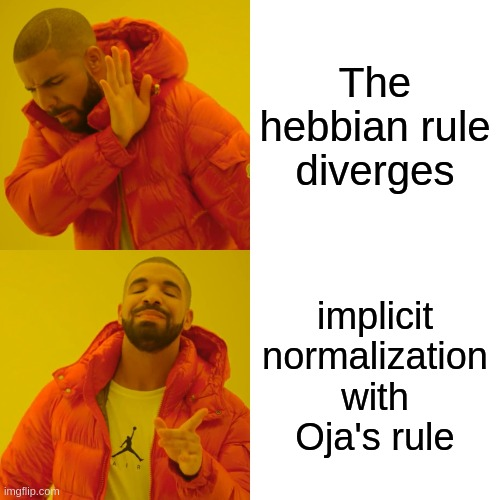
\includegraphics[width=5cm]{img/meme_oja}
    \end{center}
\end{frame}
}

\begin{frame}{\secname}

Modify the update rule such that 
\begin{itemize}
\item it contains an 
\emph{implicit normalization} to prevent divergence and 
still 
\item have $\vec w$ converge to the direction of the first PC.
\end{itemize}

\question{How?}

-By adding a \emph{decay term} to the update rule.

\begin{block}{Oja's rule:}
\begin{equation}
	\Delta \mathrm{w}_j = \varepsilon~y_{ \big( \vec{x}^{(\alpha)}; \vec{w}
		\big) } \bigg\{ 
			\underbrace{ \mathrm{x}_j^{(\alpha)} }_{
				\substack{	\text{Hebbian} \\
						\text{learning} }}
			- \underbrace{ y_{ \big( \vec{x}^{(\alpha)}; \vec{w}
				\big) } \mathrm{w}_j }_{\text{decay term}}
			\bigg\}
\end{equation}
\end{block}

\end{frame}

\subsubsection{Alternative to Oja's rule}

\mode<presentation>{   
\begin{frame}{\subsubsecname}

All Oja's rule does is:

\begin{itemize}
\item provide an
\emph{implicit normalization} to prevent divergence and 
still 
\item have $\vec w$ converge to the direction of the first PC.
\end{itemize}
	%\begin{center}
	%Dealing with the diverging hebbian rule\\
	%through implicit normalization
	\pause
	%\end{center}
    \begin{center}
		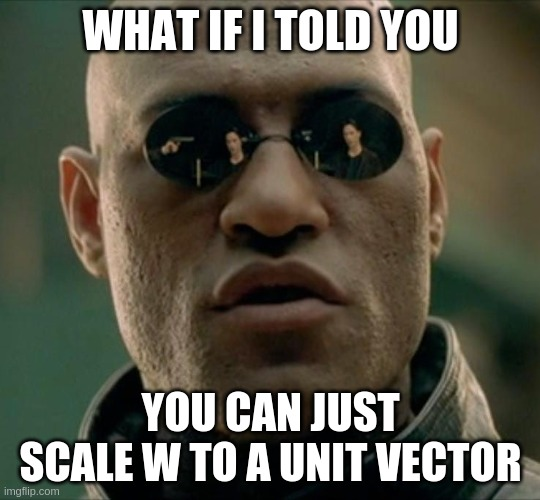
\includegraphics[width=5cm]{img/meme_normalization}
    \end{center}
\end{frame}
}


\begin{frame}{\subsubsecname}

\begin{block}{Explicit normalization} 
i.e. keep $|\vec w| = 1$ after each step by normalizing it.

\begin{equation}
	\vec{w}(t+1) = 
    \frac{\vec w(t) + \Delta \vec w}{|\vec w(t) + \Delta \vec w|} 
    = \frac
    {\overbrace{\vec{w}(t) + \varepsilon y(\vec{x}^{(\alpha)}; \vec{w}(t)) \vec{x}^{(\alpha)}}^{\text{Hebbian learning}}}
    {\underbrace{\left| \vec{w}(t) + \varepsilon y(\vec{x}^{(\alpha)}; \vec{w}(t)) \vec{x}^{(\alpha)} \right|}_{\text{Euclidean weights normalization}}}
\end{equation}

For the $j$-th component:\\
\begin{equation*}
    w_j(t+1) = \frac
    {w_j(t) + \varepsilon y(\vec{x}^{(\alpha)}; \vec{w}(t)) x_j^{(\alpha)}}
    {\sqrt{ \sum_{k=1}^{N} \left( w_k(t) + \varepsilon y(\vec{x}^{(\alpha)}; \vec{w}(t)) {x_k}^{(\alpha)} \right)^2}}
\end{equation*}
\end{block}

Keep in mind that the above explicit normalization uses the original hebbian update rule 
$\Delta \vec w = \epsilon y(\vec x^ {(\alpha)}; \vec w(t)) \vec x^{(\alpha)}$ \underline{without} the decay term. 
If we had the decay term, we wouldn't need an explicit normalization.

\end{frame}

\begin{frame}

\question{Does Oja's rule give different results than the explicit normalization?}

- No.\\

\pause

In the excercise sheet you will demonstrate that for small $\varepsilon$ the explicit normalization can be reduced to Oja's rule using a Taylor expansion around $\varepsilon = 0$ and neglecting terms of second or higher order in $\varepsilon$. 

\end{frame}
